\documentclass[10pt]{beamer}

\usetheme{metropolis}
\usepackage{appendixnumberbeamer}

\usepackage{booktabs}
\usepackage[scale=2]{ccicons}

\usepackage{pgfplots}
\usepgfplotslibrary{dateplot}

\usepackage{xspace}
\newcommand{\themename}{\textbf{\textsc{metropolis}}\xspace}

\usepackage{amsmath}
\DeclareMathOperator*{\argmin}{arg\,min}

\title{Mid-term Project}
\subtitle{Chan and Ho: A Simple and Efficient Estimator for Hyperbolic Location System}
\date{\today}
\author{Zhang Niansong\quad(16308149) \\ Yang Songyi\quad(16308131)}

\begin{document}

\maketitle

\begin{frame}{Table of contents}
  \setbeamertemplate{section in toc}[sections numbered]
  \tableofcontents[hideallsubsections]
\end{frame}

\section{Introduction}

\begin{frame}{Position Fix by TDOA}
  \begin{columns}[T,onlytextwidth]
    \column{0.6\textwidth}
      \begin{itemize}
        \item Assuming a source is emitting signal in all directions
              and an array of sensors are picking up the signal,
              it will arrive at different sensors at different time.
        \item \textbf{TDOA :} \textit{Time Difference Of Arrival}
        \item Then the location of the source can be estimated
              by measuring the delay of signal arriving at different sensor.
      \end{itemize}
    \column{0.3\textwidth}
      \begin{figure}[t]
        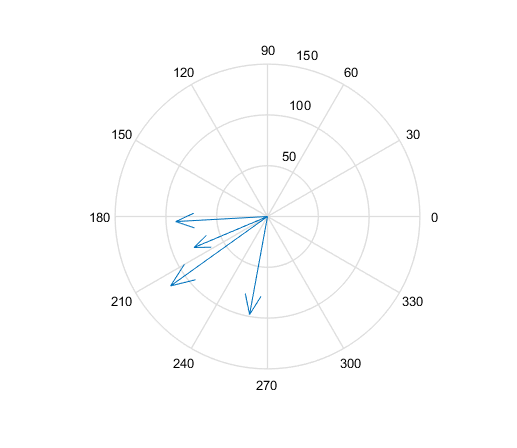
\includegraphics[width=1\textwidth]{intro.png}
        \caption{Sensors and source.}
      \end{figure}
  \end{columns}
\end{frame}

\begin{frame}{Position Fix by TDOA: Noise}
  Vector of \textbf{TDOA}:
    $$\bf{d} = \begin{bmatrix} d_2-d_1 & d_3-d_1 & \cdots \end{bmatrix}^\it{T}$$
  However, 100\% precise measurement of \textbf{TDOA} is not possible.
  Noise is always present.

  Naturally, the noise in \textbf{TDOA} is a \textit{multivariate Gaussian distribution}
  centered at true value, with covariance given by matrix:
    $$ \mathbf{Q} = \sigma^2
      \begin{bmatrix}
        1 & 0.5 & \cdots & 0.5 \\
        0.5 & 1 & \cdots & 0.5 \\
        \vdots & \vdots & \ddots & \vdots \\
        0.5 & 0.5 & \cdots & 1 \end{bmatrix}
    $$
    where $\sigma^2$ is the noise power.
\end{frame}

\section{Propsed Method}

\begin{frame}{Proposed Method}
  \begin{itemize}[<+- | alert@+>]
    \item By assuming $x, y$ and $r_1$ are independent, the non-linear
          equations can be reduced into linear ones.

    \item Given different situations, use \emph{Maximum Likelihood} (ML)
          estimator to solve the linear equations.

    \item Incorporate the dependent relationship back into the solution (if necessary)
          to get more accurate solution.

  \end{itemize}
\end{frame}

\begin{frame}{Proposed Method: Workflow}

  \begin{figure}
    \centering
    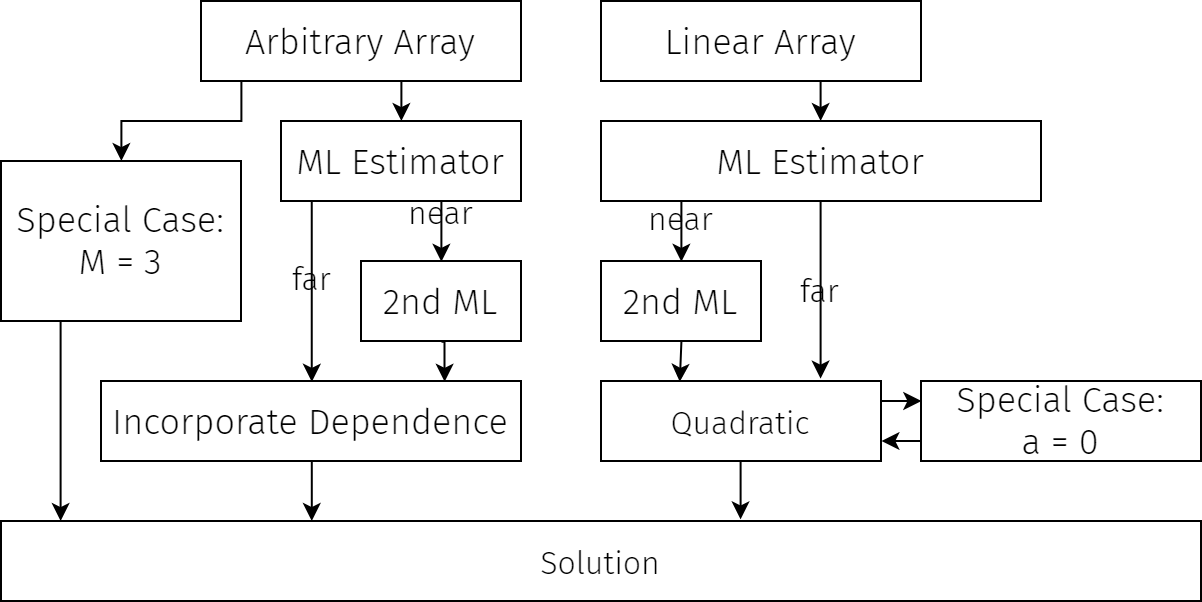
\includegraphics[width=0.9\textwidth]{proposed-workflow.png}
    \caption{Flowchart of the proposed method.}
  \end{figure}
\end{frame}

\begin{frame}{Proposed Method: Arbitrary Array}
  "Arbitrary" refers to that sensors are arranged in a non-linear manner,
  thus avoiding singularity during computation.
  \begin{itemize}
    \item With \alert{3} sensors ($M = 3$), system is not overdetermined.
            $$\mathbf{z}_p = - \begin{bmatrix}x_{2,1}&y_{2,1} \\ x_{3,1}&y_{3,1}\end{bmatrix}^{-1} \times
              \begin{Bmatrix} \begin{bmatrix}r_{2,1}\\r_{3,1}\end{bmatrix}r_1 + \frac{1}{2}
                              \begin{bmatrix}r_{2,1}^2-K_2+K_1 \\ r_{3,1}^2-K_3+K_1 \end{bmatrix}\end{Bmatrix}$$
            $$r_1^2 = K_1-
              2\begin{bmatrix}x_1&y_1\end{bmatrix} \mathbf{z}_p+
              \mathbf{z}_p^T \mathbf{z}_p$$
          where $K_i = x_i^2 + y_i^2, \mathbf{z}_p = \begin{bmatrix}x&y\end{bmatrix}^T$.
    \item Therefore, the solution can be found simply by
    \begin{enumerate}
      \item solving a quadratic equation of $r_1$;
      \item insert $r_1$ back and solve the linear equation groups of $x$ and $y$.
    \end{enumerate}
  \end{itemize}
\end{frame}

\begin{frame}{Proposed Method: Arbitrary Array (cont'd)}
  \begin{itemize}
    \item With more than 3 sensors, the system is overdetermined.
    \item Here we denote:
            $$\mathbf{h}= \frac{1}{2}
              \begin{bmatrix}r_{2,1}^2-K_2+K_1 \\
                             r_{3,1}^2-K_3+K_1 \\
                             \vdots \\
                             r_{M,1}^2-K_M+K_1\end{bmatrix}$$
            $$\mathbf{G}_a=-
              \begin{bmatrix} x_{2,1} & y_{2,1} & r_{2,1} \\
                              x_{3,1} & y_{3,1} & r_{3,1} \\
                              \vdots  & \vdots  & \vdots  \\
                              x_{M,1} & y_{M,1} & r_{M,1} \end{bmatrix}$$
            $$\mathbf{B}= \textbf{diag} \{r_2^0,r_3^0,\cdots,r_M^0\}$$
    \item
  \end{itemize}
\end{frame}

\begin{frame}{Proposed Method: Arbitrary Array (cont'd)}
  \begin{itemize}
    \item Using ML estimator, $\mathbf{z}_a=\begin{bmatrix}x\\y\\r_1\end{bmatrix}$ can be obtained as
          $$\begin{align}
            \mathbf{z}_a&=\argmin\{(\mathbf{h}-\mathbf{G}_a\mathbf{z}_a)^T
                                    \Psi^{-1}(\mathbf{h}-\mathbf{G}_a\mathbf{z}_a)\}\\
                        &=(\mathbf{G}_a^T\Psi^{-1}\mathbf{G}_a)^{-1}\mathbf{G}_a^T\Psi^{-1}\mathbf{h}
            \end{align}$$
    \item When the emitter is far away from the sensors,
          and since scaling of $\Psi$ do not effect the solution
          $\mathbf{z}_a$can be approximated as
          $$\mathbf{z}_a\approx(\mathbf{G}_a^T\mathbf{Q}^{-1}
            \mathbf{G}_a)^{-1}\mathbf{G}_a^T\mathbf{Q}^{-1}\mathbf{h}$$
    \item When the source is nearby, its location can still be approximated
          using $\mathbf{Q}$, and using one iteration to improve accuracy.
  \end{itemize}
\end{frame}

\begin{frame}{Proposed Method: Dependency of Arbitrary Array}
  \begin{itemize}
    \item The next step is to consider the dependency between $x$, $y$ and $r_1$.
    \item Again using ML, we have
          $$\mathbf{z}_a^{'}=(\mathbf{G}_a^{'T}\Psi^{'-1}\mathbf{G}_a^{'})^{-1}
                              \mathbf{G}_a^{'T}\Psi^{'-1}\mathbf{h}^{'}$$
          where
          $$\mathbf{h}^{'}=\begin{bmatrix}(x-x_1)^2\\(y-y_1)^2\\r_1^2\end{bmatrix},\quad
            \mathbf{G}_a^{'}=\begin{bmatrix}1&0\\0&1\\1&1\end{bmatrix}$$
          and
          $$\Psi^{'}=4\mathbf{B}^{'}(\mathbf{G}_a^{0T}\Psi^{-1}\mathbf{G}_a^0)^{-1}\mathbf{B}^{'},\quad
            \mathbf{B}^{'} = \textbf{diag} \{x-x_1,y-y_1,r_1^0\}$$
  \end{itemize}
\end{frame}

\begin{frame}{Proposed Method: Solution of Arbitrary Array}
  \begin{itemize}
    \item Similar simplification can be made when the source is far away,
          by subsitituding $\Psi$ with $\mathbf{Q}$.
    \item After acquiring $\mathbf{z}_a^{'}$, we have
          $$\mathbf{z}_a^{'}=
            \begin{bmatrix}(x^0-x_1)^2\\(y^0-y_1)^2\end{bmatrix}$$
    \item Then $x^0$ and $y^0$ can be canculated by taking square roots of the positive values.
  \end{itemize}
\end{frame}

\begin{frame}{Proposed Method: Linear Array}
  If the sensors are arranged linearly, i.e. on a line, then the positions
  can be described by $$y=ax+b$$

  Here the procedure used for \emph{Arbitrary Array} would fail due to matrix singularity.

  However, a similar solution can be developed with slight modifications.
\end{frame}

\begin{frame}{Proposed Method: Linear Array (cont'd)}
  \begin{itemize}
    \item Taking the relationship $y=ax+b$, rewrite $\mathbf{z}_a$ and $\mathbf{G}_a$
          as
          $$\mathbf{z}_l=\begin{bmatrix}x+ay\\r_1\end{bmatrix},\quad
            \mathbf{G}_l=-\begin{bmatrix}
                          x_{2,1} & r_{2,1}\\
                          x_{3,1} & r_{3,1}\\
                          \vdots  & \vdots \\
                          x_{M,1} & r_{M,1}\end{bmatrix}$$
    \item We can have something very similar to that in arbitrary array
          $$\mathbf{z}_l=(\mathbf{G}_l^T\Psi^{-1}\mathbf{G}_l)^{-1}\mathbf{G}_l^T\Psi^{-1}\mathbf{h}$$
          where $\Psi$ and $\mathbf{h}$ are the same as in arbitrary Array.
    \item Similar approach of taking $\mathbf{Q}$ for $\Psi$ and use of iteration can be applied here.
  \end{itemize}
\end{frame}

\begin{frame}{Proposed Method: Solution of Linear Array}
  We now have $\mathbf{z}_l=\begin{bmatrix}x+ay\\r_1\end{bmatrix}$,
  denoted as $\mathbf{z}_l=\begin{bmatrix}w\\r_1\end{bmatrix}$.
  \begin{itemize}
    \item $y$ and $x$ can be solved through quadratic equation
          $$y=\frac{-E\pm\sqrt{E^2-4AC}}{2A},\quad x=w-ay$$
          where$$A=1+a^2,E=-2(aw+b),C=K_1-2x_1w+w^2-r_1^2$$
    \item When $a=0$, the solution becomes
          $$y=\pm\sqrt{r_1^2-(w-x_1)^2}+y_1,\quad x=w$$
  \end{itemize}
\end{frame}

\end{document}
